\documentclass[11pt]{article}
\usepackage{amsthm,amsfonts,amssymb,amsmath}
\usepackage{tikz}
\usetikzlibrary{positioning}
% Optional PGF libraries
\usepackage{pgflibraryarrows}
\usepackage{pgflibrarysnakes}
\usepackage[top=1in, bottom=1in, left=1.25in, right=1.25in]{geometry}
\usepackage{enumerate}
\usepackage[colorlinks,linkcolor = black, anchorcolor = black,citecolor = black]{hyperref}

\author{Zihao Wang\footnote{N-number: N11385738, NetID: zw1074}
	}
\title{\textbf{Solution for Problem Set 4}}
\renewcommand{\P}{\mbox{P}}
\begin{document}
	\maketitle
	\section*{Problem 1}
	\subsection*{A}
	\begin{align*}
		\P(D = T) &= \sum_{S}^{}\sum_{T}\P(D=T|S,T)\P(S,T)\\
		&= 0.95\times 0.75\times 0.6 + 0.1\times 0.75\times 0.4 + 0.2\times 0.6\times 0.25\\
		&= \frac{39}{80}\\
		\P(D = F) &= 1-\P(D = T) = \frac{41}{80}
	\end{align*}
	\subsection*{B}
	\begin{align*}
		\P(L=T|D=F) &= \frac{\P(L=T,D=F)}{\P(D=F)}\\
		&= \frac{\P(L=T,D=F,S=T) + \P(L=T,D=F,S=F)}{\P(D=F)}\\
		&= \frac{0.05\times 0.6\times 0.75 + 0.9\times 0.4 \times 0.75}{\frac{41}{80}}\\
		&= \frac{117}{205}
	\end{align*}
	\subsection*{C}
	\begin{align*}
		\P(D2=T|D1=F) &= \frac{\P(D2=T,D1=F)}{\P(D1)}\\
		&= \frac{\sum_{S2,L}^{}\P(D2,D1|S2\cap L)\P(S2\cap L)}{\P(D1)}\\
		&= \frac{\sum_{S2,L}^{}\P(D2|S2\cap L)\P(D1|S2\cap L)\P(S2)\P(L)}{\P(D1)}\\
		&= \frac{\sum_{S2,L}^{}\P(D2|S2\cap L)\P(S2)\sum_{S1}^{}\P(D1|L,S1)\P(L,S1)}{\P(D1)}\\
		&= 0.399659
	\end{align*}
	\subsection*{D}
	\begin{figure}[!htbp]
		\centering 
		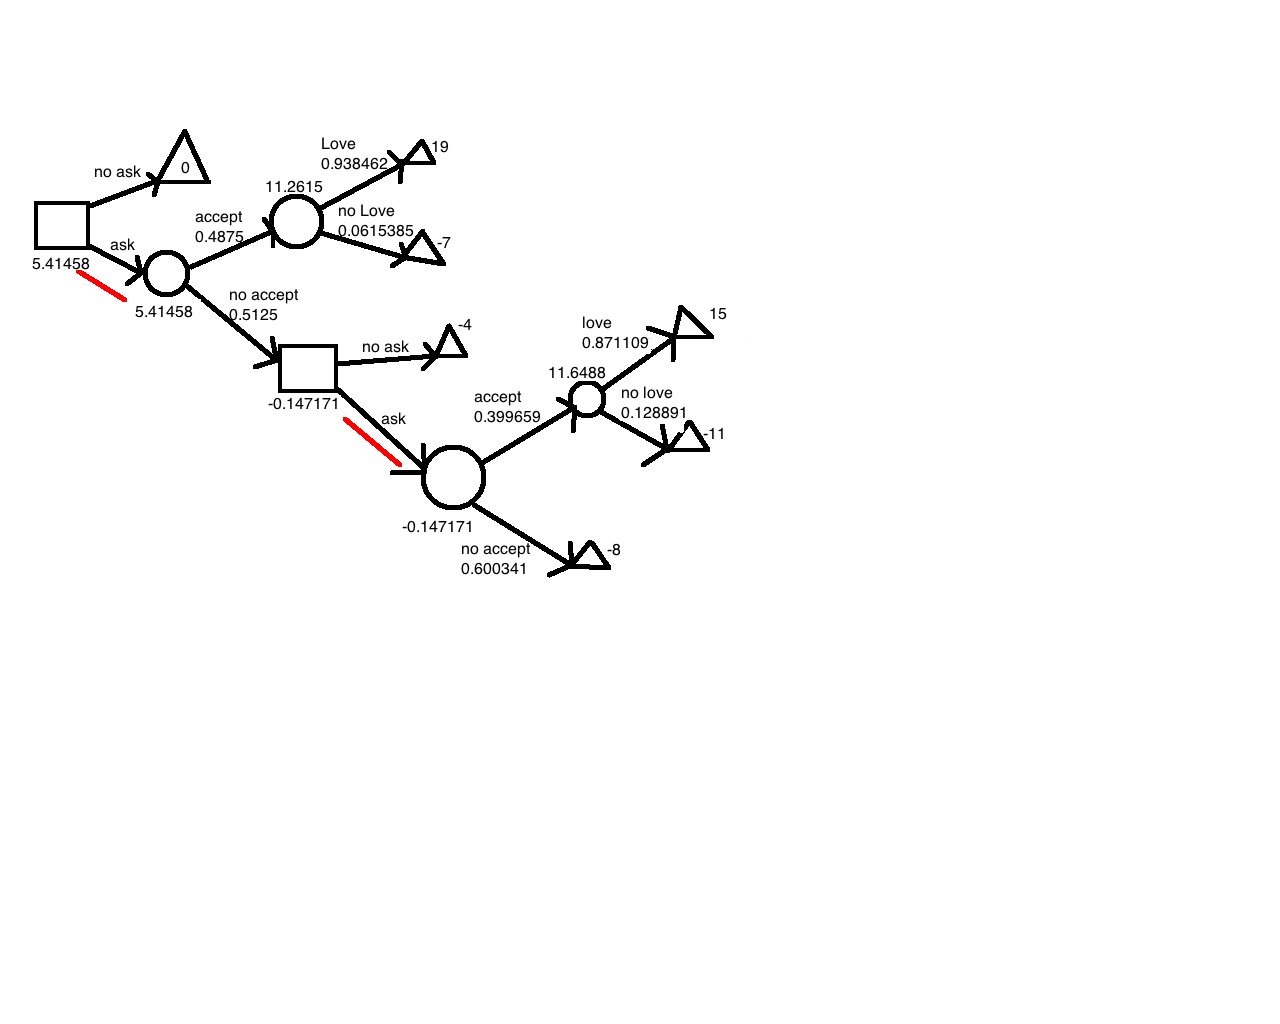
\includegraphics[height=18cm ,width=20cm]{Untitled.png}
		\caption{Diagram for \textbf{Problem 1}} \label{figure7}
	\end{figure}
	\section*{Problem 2}
	\subsection*{A}
	Let $ X_i $ be the variable of the outcome of i-th clause, 0 for false and 1 for truth. Then the sum of them is $ K $. Then
	\begin{align*}
		E(K) = \sum_{i=1}^{N}E(X_i) = \frac{7N}{8}
	\end{align*}
	\section*{B}
	When enumerate all possible value, the result is:
	\begin{itemize}
		\item $ K=5 $ has 8 possible values.
		\item $ K=4 $ has 6 possible values.
		\item $ K=3 $ has 2 possible values.
		\item $ K=2,1,0$ has no value.
	\end{itemize}
	So the distribution of $ K $ is
	\begin{align*}
		\P(K=5) = \frac{1}{2}, \P(K=4) = \frac{3}{8}, \P(K=3) = \frac{1}{8}
	\end{align*}
\end{document}